\documentclass[twocolumn,english,notitlepage]{article}
\usepackage[margin=0.5in]{geometry}
\setlength{\parindent}{0pt} % no indents

% Math
\usepackage{amsmath}
\usepackage{physics}
\usepackage{amsfonts} % for mathbb

% Citetations
\usepackage[ backend=bibtex, sorting=none, autocite=plain]{biblatex}
\addbibresource{refs/references}
\usepackage{xcolor}
\usepackage{hyperref}
\hypersetup{
    colorlinks,
    linkcolor={red!50!black},
    citecolor={blue!50!black},
    urlcolor={blue!80!black}}


% Formatting
\usepackage{float}
\usepackage{graphicx}
\usepackage{subcaption}

\graphicspath{ {./figs/} } 

% Misc
\usepackage{appendix}
\usepackage{xfrac} % provides \sfrac

% Commands

\newcommand{\comment}[1]{\textcolor{red}{#1}\\}

\newcommand{\integral}[1]{\ensuremath{\int\!\mathrm{d}#1\,}}
\renewcommand{\d}[2][x]{\ensuremath{\frac{\mathrm{d}#2}{\mathrm{d}#1}}}

\renewcommand{\vec}[1]{\boldsymbol{#1}}
\newcommand{\pclosed}[1]{\left(#1\right)}
\newcommand{\bclosed}[1]{\left[#1\right]}
\newcommand{\cclosed}[1]{\left\{#1\right\}}
\newcommand{\vclosed}[1]{\left|#1\right|}
\renewcommand{\norm}[2][]{\ensuremath{\|#2\|_{#1}}}
\renewcommand{\exp}[1]{e^{#1}}
\newcommand{\exptext}[1]{\operatorname{exp}\pclosed{#1}}
\newcommand{\dimof}[1]{\bigl[#1\bigr]}

\renewcommand{\expval}{\operatorname{\mathbb{E}}}
\renewcommand{\var}{\operatorname{Var}}
\newcommand{\bias}{\operatorname{Bias}}
\DeclareMathOperator{\eye}{\mathbb{I}}
\DeclareMathOperator{\sgn}{sgn}

\newcommand{\betahat}{\hat{\beta}}
\newcommand{\msub}[2]{\ensuremath{{#1}_\text{#2}}}

\title{Bias-variance tradeoff in simple linear models} % very much working title
\author{Anna Aasen, Carl Martin Fevang, Håkon Kvernmoen}
\date{\today}

\begin{document}

\twocolumn[
    \begin{@twocolumnfalse}
        \maketitle
        \begin{abstract}
            This is the abstract.
        \end{abstract}
    \end{@twocolumnfalse}
]

\section{Introduction}
    In this project, we will introduce some of the most important general properties of machine learning models in the context of linear regression. Specifically the mean squared error (MSE), the bias, and the variance of data predictions are essential in evaluating the quality of a statistical model. We look at the phenomena of underfitting and overfitting, and explore them in the context of bias-variance trade-off. The three models we will use explicitly are Ordinary Linear Regression (OLS), Ridge regression and Least-Absolute-Shrinkage-and-Selection-Operation (LASSO) regression. These will first be tested on the 2D Franke function, and later on real geographical terrain data.

    The aforementioned models will be explored using resampling techniques, which will be employed to extract the relevant statistical quantities in an accurate way. We will use the standard methods of Bootstrapping and Cross Validation and compare the results we get between them across the three linear models.

    All the models will be applied by fitting a two-dimensional polynomial expansion to the observed data.



\begin{figure}[H]\label{fig:intro:plat}
    \centering
    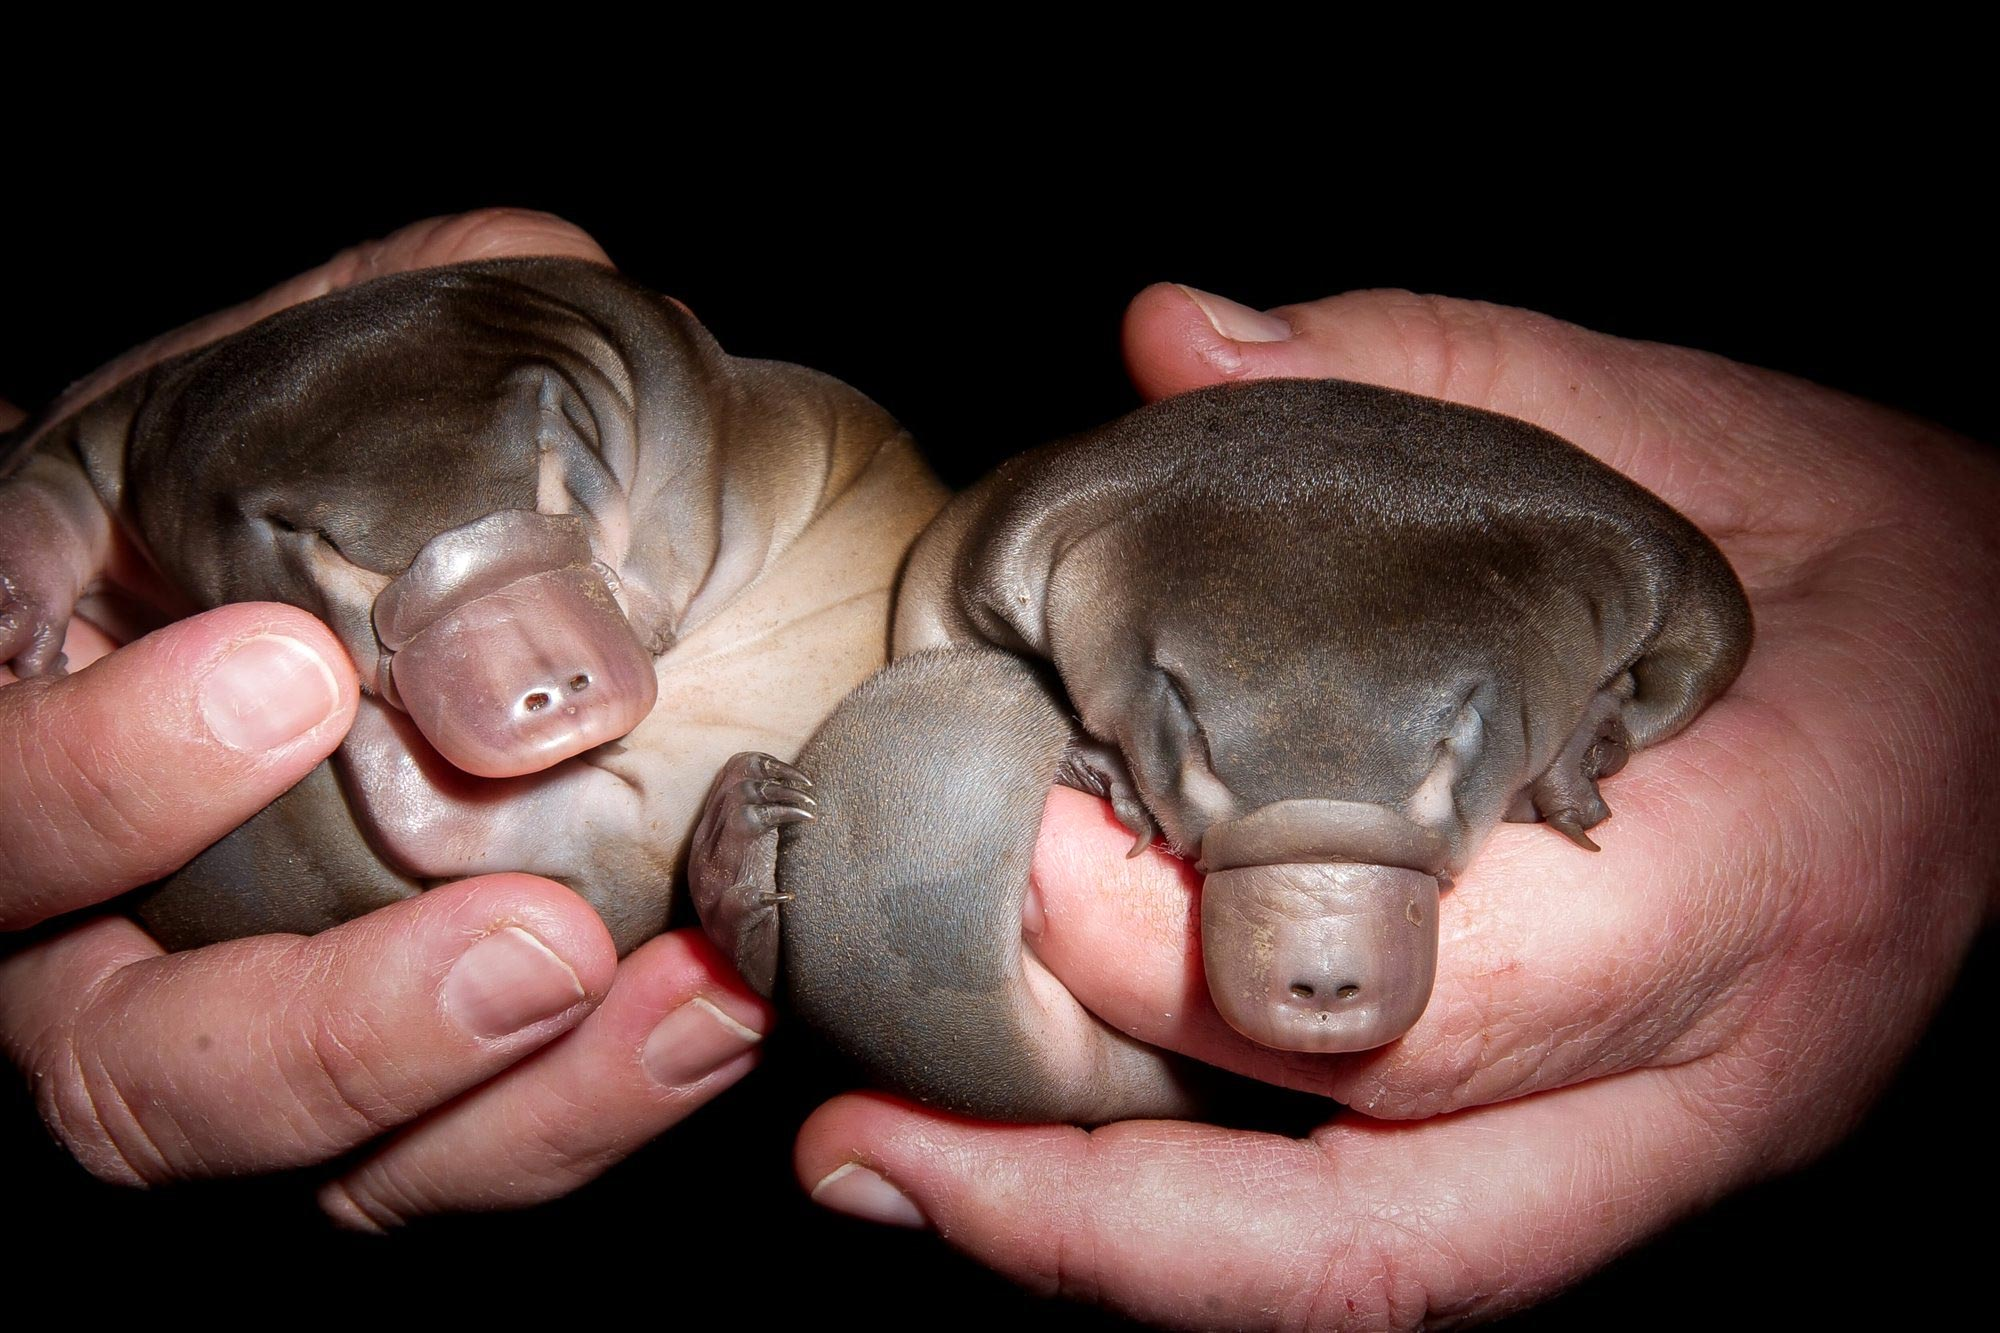
\includegraphics[width=0.5\linewidth]{Young-Platypus.jpg}
    \caption{Some figure caption}
\end{figure}

\section{Theory}
    Before we delve into to details of the theory section, it is useful to take a moment to define the quantities we will be dealing with. Let $\vec{y}$ denote a vector of a series of measured values $y_i$, $i\in 1, 2,..., n$ at points $X$, where $X$ is a matrix where the rows $x_i$ correspond to the input values that produced the measurement $y_i$. For completeness we refer to the columns of $X$ as $\vec{x}_a$, $a=1, 2,..., p$.\footnote{Throughout this project, $a, b$ will always index the $p$ features for a model, and $i, j$ the $n$ data points.} Together, these form the dataset $\mathcal{D} = \vclosed{(y_i, x_i)}$. Another important set of values is $\vec{\theta}$ which contains the parameters that will define the model we will use to predict the data.

    We will assume that the measurements $y_i$ are generated from an exact function $f(x)$ with stochastic noise $\epsilon$ added, such that $y_i = f(x_i) + \epsilon$. Throughout this project, we will assume that the noise is normally distributed with mean 0 and some standard deviation (std) $\sigma$; $\epsilon \sim \operatorname{N}(0,\sigma^2)$. Furthermore, we will assume that the noise between different measurements is independent and identically distributed (i.i.d.). Our job then is to model an $\hat{f}(x)$ that we want to be close to $f(x)$.

    \subsection{Error assesement and model optimisation}
        When we want to create a statistically informed model that is able to predict future measurements, we need to develop a metric for how well our model fits the data we already have. That is, we want to optimise our parameters $\vec{\theta}$ such that $\hat{f}(x) \approx f(x)$.
        %MSE and R2?? Can Bias and Variance also be included here?? -Anna

    \subsection{Statistical introduction to linear regression}
        A way to motivate the process of statistical learning is that we want to develop a process by which we use observed data to inform our belief in a future outcome. Such a process can be developed from the ideas of Bayes' theorem, which we can use to inform us what confidence we should have in the parameters of a given model, given data points we have observed.
        
        Bayes' theorem tells us that our \textit{posteriori} confidence in $\vec{\theta}$, given the available data, is given by the probabilty
        \begin{align}
            P(\vec{\theta}|X, \vec{y}) = \frac{P(\vec{y}|X,\vec{\vec{\theta}})P(\vec{\theta})}{P(X,\vec{y})},
        \end{align}
        where $P(\vec{y}|X, \vec{\theta})$ is the \textit{likelihood}, and $P(\vec{\theta})$ is our \textit{prior} confidence in $\vec{\theta}$. $P(X,\vec{y})$ plays the role of a normalisation, and can safely be ignored -- either because we look for values of $\vec{\theta}$ that maximise the probability, or because we assume the probabilities $P(\vec{y}|X,\vec{\theta})$ and $P(\vec{\theta})$ which we then can properly normalise. Now we have a framework through which we can build a model by making assumptions about the probability distributions $P(\vec{y}|X,\vec{\theta})$ and $P(\vec{\theta})$ to give us a probability distribution for the parameters $\vec{\theta}$ that we can maximise.


        \subsubsection{Ordinary least squares}
            Now we can define the ordinary least squares method by assuming that the data $y$ that we want to make a fit to has a linear noise term that is normally distributed with mean nought. That is, the data is generated as $y(x) = f(x) + \epsilon$, where $f(x)$ is some analytic, non-stochastic function of the data input $x$, and $\epsilon \sim N(0, \sigma^2)$. Further, if we make a model fitting $y(x)$ by a $\hat{y}(x)$, we should expect the error at every data point $(y_i, x_i)$ to be be normally distributed with the same variance, i.e., independently and identically distributed (i.i.d.). This can be summarised
            \begin{align}
                P(\vec{y}|X, \vec{\theta}) = \prod_{i=1}^{n} \frac{1}{\sqrt{2\pi\sigma^2}} \exp{-\frac{{(y_i-\hat{y}_i)}^2}{2\sigma^2}}.
            \end{align}
            Furthermore, we assume the parameters $\vec{\theta}$ to be distributed evenly, and as such, $P(\vec{\theta})$ just contributed to an overall normalisation. This means that maximising $P(\vec{y}|X, \vec{\theta})$ amounts to the same as maximising $P(\vec{\theta}|X, \vec{y})$, and can be done analytically.

            Knowing that the Gaussian distribution has a single extremum that is a maximum, we can find the values for $\vec{\theta}$ maximising the probability as
            \begin{align} \nonumber
                \d[\theta_k]{P(\vec{y}|X,\vec{\theta})} &= 0 \\
                \Rightarrow \prod_{i=1}^{n} \frac{1}{\sqrt{2\pi\sigma^2}} \frac{1}{\sigma^2} X_{ib}(y_i-X_{ia}\theta_a) \exp{-\frac{{(y_i - X_{ia}\theta_a)}^2}{2\sigma^2}} &= 0,
            \end{align}
            which as we can see, is maximisable point by point. This means that the optimal parameters $\msub{\vec{\hat{\theta}}}{OLS}$ that maximise $P(\vec{y}|X, \vec{\theta})$ can be found as
            \begin{align}
                \boxed{
                \msub{\vec{\hat{\theta}}}{OLS} = \pclosed{X^TX}^{-1} X^T \vec{y}.
                }
            \end{align}

%Should this be a subsubsection? -Anna
        \subsection{Ridge and LASSO regression}
            So far, we have assumed that the parameters $\vec{\theta}$ are uniformly distributed, and as such have no \textit{bias} towards any particular value. In practice, this means that the OLS model will contort to fit itself to all values in the data. As such, a motivation for adding a bias could be for the sake of stability in the fit. These methods are called \textit{regularised} methods. An example is ridge regression, where one assumes that the parameters are normally distributed, such that parameter values far from the mean are thought less likely to occurr. This in practice means that the model is less willing to contort to outliers in the dataset, trading it for a bias towards certain parameter values. Assuming the probability distrbution for $\vec{\theta}$
            \begin{align}
                P(\vec{\theta}) = \prod_{a=1}^{p} \frac{1}{\sqrt{2\pi\tau^2}} \exp{-\frac{\theta_a^2}{2\tau^2}},
            \end{align}
            with a derivative with respect to $\theta_b$
            \begin{align}
                \d[\theta_b]{P(\vec{\theta})} = -\prod_{a=1}^{p} \frac{1}{\sqrt{2\pi\tau^2}} \frac{1}{\tau^2} \theta_b \exp{-\frac{\theta_a^2}{2\tau^2}} = -\frac{1}{\tau^2} \theta_b P(\vec{\theta}),
            \end{align}
            the condition for maximising $P(\vec{\theta}|X, \vec{y})$ becomes
            \begin{align} \nonumber
                \d[\vec{\theta}]{P(\vec{y}|X, \vec{\theta})} P(\vec{\theta}) + P(\vec{y}|X, \vec{\theta}) \d[\vec{\theta}]{P(\vec{\theta})} &= 0 \\
                \pclosed{ \frac{1}{\sigma^2} X^T(\vec{y}-X\vec{\theta}) - \frac{1}{\tau^2} \vec{\theta} } P(\vec{y}|X,\vec{\theta}) P(\vec{\theta}) &= 0.
            \end{align}
            Rewriting with a parameter $\lambda = \sigma^2/\tau^2$, the optimal parameters $\msub{\vec{\hat{\theta}}}{ridge}$ are given by
            \begin{align}
                \boxed{
                \msub{\vec{\hat{\theta}}}{ridge} = \pclosed{X^TX + \lambda \eye}^{-1} X^T \vec{y}.
                }
            \end{align}
            This has the added bonus of ensuring that $X^TX + \lambda \eye$ is always invertible, as $\det(\lambda \eye) \neq 0$ for $\lambda>0$.


            LASSO regression builds on the same ideas as ridge regression, by assumes rather a Laplace distribution $L(0, \tau)$ for the parameters $\vec{\theta}$. This gives
            \begin{align}
                P(\vec{\theta}) = \prod_{a=1}^{p} \frac{1}{2\tau} \exp{-\frac{|\theta_a|}{\tau}},
            \end{align}
            which as we can see is not differentiable at $\theta_i = 0$. This means that the optimisation of this the probability $P(\vec{\theta}|X, \vec{y})$ is not necessarily possible analytically without putting bounds on the data $X, \vec{y}$, and even numerical algorithms like gradient descent will encounter run into trouble. Furthermore, it is not optimisable point by point, unless bounds like $X^TX$ being diagonal are enforced, which makes LASSO generally less used. Nevertheless, we can coax a cost function out of the probability that is minimalisable. Letting the cost function be written $\msub{C}{lasso}(\vec{\theta}) = -A\log\pclosed{P(\vec{\theta|X,\vec{y}})} + B$  we can choose the constants $A, B$ such that
            \begin{align}
                \boxed{
                    \msub{C}{lasso}(\vec{\vec{\theta}}) = \norm[2]{ \vec{y} - X\vec{\theta} }^2 + \lambda \norm[1]{\vec{\theta}},
                }
            \end{align}
            where $\lambda = \frac{2\sigma^2}{\tau}$ and $\norm[p]{\vec{v}} = \pclosed{\sum_k |v_k|^p}^{\sfrac{1}{p}}$ denotes the $L_p$ norm of the vector $\vec{v} \in \mathbb{R}^k$.

    % Should we at some point mention the hessian matrix and the C of Ridge being convex (Hessian is positive definite) -Anna

\section{Method}
Something general about initially fitting Franke data using OLS, ridge and lasso. Then moving on to real terrain data something something.
    
    \subsection{Franke function}

    For the initial testing of our implemented fitting routines, we will use the so called \textit{Franke function}. Being able to control the number of sample points and noise levels will serve as a good examination of our models advantages and disadvantaged. Defined for $x, y \in [0,1]$

    \begin{align}
        F(x,y) = f_1(x,y) + f_2(x,y) + f_3(x,y) + f_4(x,y) + \epsilon \label{eq:met:Franke_Function}
    \end{align}

    Where the $f_i(x,y)$ are Gaussian functions, constructed to mimic the shape of a hill top landscape. More concretely, these are defined as:

    \begin{align} \nonumber
        f_1(x,y) &= \frac{3}{4}\exptext{ -\frac{(9x-2)^2}{4} - \frac{(9y-2)^2}{4} } \nonumber \\
        f_2(x,y) &= \frac{3}{4}\exptext{ -\frac{(9x+1)^2}{49} - \frac{(9y+1)}{10}} \nonumber \\
        f_3(x,y) &= \frac{1}{2}\exptext{ -\frac{(9x-7)^2}{4} - \frac{(9y-3)^2}{4}} \nonumber \\
        f_4(x,y) &= -\frac{3}{4}\exptext{ -(9x-4)^2 - (9y-7)^2} \nonumber
    \end{align}

    And $\epsilon$ is some stochastic noise $\epsilon \sim N(0,\sigma^2)$. By visual inspection, we can fine tune $\sigma$ to create data that looks like noisy digital terrain data.
    
    \subsection{Linear regression}
    \comment{not sure about how we should divide these subsections, but I wanted to write a bit about data scaling}
    Before fitting the regularised models to the sampled data, we will scale the data using the $Z$-score normalisation. This scales the inputs $x_i$ and the targets $\vec{y}$ such that they have a mean value of $0$ with a standard deviation $1$. In effect, we rescale
    \begin{subequations}
        \begin{align}
            \vec{y}^\text{scaled} &= \frac{\vec{y}-\bar{y}}{\bar{\sigma}_{\vec{y}}}, \\
            \vec{x}_a^\text{scaled} &= \frac{\vec{x}_a - \bar{x}_a}{\bar{\sigma}_{\vec{x}_a}},
        \end{align}
    \end{subequations}
    where $\bar{z} = \frac{1}{n} \sum_{i=1}^n z_n$ detotes the sample mean of $\vec{z}$ and $\sigma_{\vec{z}}^2 = \frac{1}{n} \sum_{i=1}^n {(z_i-\bar{z})}^2$ denotes the sample std of $\vec{z}$.

    \subsection{Resampling techniques}
    With the intent to compute more accurate measures for goodness of fit (such as MSE and $R^2$) to evaluate our model, we 
    artificially increase the data sample by repeatedly fitting the model on subsamples of our data. This approach is called resampling and consists of a variety of methods. In this project we have utilized \textit{Bootstrapping} and \textit{k-fold Cross-validation}. 

        \subsubsection{Bootstrap}
        The method of bootstrapping consists of creating a so-called bootstrapped dataset where the data points are sampled with replacement from the original sample. Then the model is trained and the relevant measures for goodness of fit calculated on the bootstrapped data. This process is repeated a certain number of times. The mean of the measures is then calculated across the bootstrapped models. Through the central limit theorem this mean is assumed to be the more accurate measure for goodness of fit and therefore a better evaluation of our model.  

        \subsubsection{Cross-validation}
        With the intent to compute more accurate measures for goodness of fit (such as MSE and $R^2$), we 
        artificially increase the data sample by fitting the model on partitioned subsamples (which we will call \textit{folds}). Using some folds
        for fitting the model and others for computing metrics, we can get multiple values for the same measure by changing which folds are used for fitting 
        and which are used for calculating measures. This is the basic idea of cross validation.
        \newline\newline
        In this report, we will use the famouse \textit{k-fold Cross-validation} technique. Consider a data sample $D = (\vec{y}, X)$, consisting of $n$ data points. Initially we partion $D$ into $k$ folds $D_i$, $i = 1, ... , k$ of equal size.   
        For each fold $D_i$, a model is fitted using every fold \textit{except} $D_i$, which we write as $D_{-i}$. With this model, we calcualte the different measures 
        using $D_i$, which was not used to fit the model. When this is done for all $k$ folds, we take the mean of the measures to get the 
        final goodness of fit. 


\section{Results}

\section{Discussion}
    \subsection{Data scaling}
        \comment{This should probably be a subsubsection within something else. Just summing up the thoughts we have thrown around regarding the necessity and function of scaling.}
        \comment{Please read and see if it makes sense at all!}
        The scaling of the inputs and measurments can roughly be divided into two operations, each with their own set consequences. Let us first consider shifting of the measurements $\vec{y}$ and the inputs $\vec{x}_a$ by their respective means. Effectively, this eliminates a degree of freedom from our model $\hat{f}(x)$ as we set its mean value to nought, and leave out any parameter that would govern the intercept $\hat{f}(0)$. However, if we shift $\vec{y}$ to have a mean of nought as well, this degree of freedom becomes redundant, and we end up effectively reducing the dimensionality of the model by one. Moreover, in regularised models where some norm of the parameters $\norm[p]{\vec{\theta}}$ is penalised, we remove any penalisation of the choice of the intercept. This is natural to do, as the goal of these methods is to reduce the variance of the model, something which is not affected by changing the intercept.

        Considering now the rescaling of $\vec{y}$ and $\vec{x}_a$, these affect the fitting of the model more subtely. Looking at it through the lense of dimensionality know that
        \begin{align}
            \dimof{\theta_a} = \dimof{y} / \dimof{x_a}.
        \end{align}
        From this we can infer that the order of magnitude of a parameter $\theta_a$ is governed by the dimension its corresponding feature $\dimof{x_a}$. This matters in the regularised models where a cost is associated with the norm of the parameters $\norm[p]{\vec{\theta}}$, which will be dominated by parameters whose dimension is large. In practice, this means that the fitting will focus more on reducing the magnitude of the parameters whose associated dimension is large, letting the others fluctuate more freely. By making the $x_a$'s dimensionless, the parameters are put on a `level playing field', so to speak. The dimension of $y$ serves to raise or lower the order of magnitude of the all the parameters equally, and can be adjusted as to avoid numerical truncation errors by avoiding larger floats.


    \subsection{Resampling}
        \comment{Here I am just writing a bit on our discussion about the limit of resampling. Structure of the discussion section is very much not set in any stone.}
        Resampling a given data set seems on the face of it to be truly the work of magic. Somehow we invoke the law of large samples from the central limit theorem (\comment{needs to be added}) that our statistical quantities, like the mean value, approaches the true value as the sample size grows. However, that is not exactly what we are doing when we are resampling. To illustrate this, we can think of a coin-flipping experiment where are results are categorically heads or tails. If we perform the experiment an \textit{odd} number of times, we must necessarily end up with either more heads or more tails. If we then continously resample from this dataset, a mean value should by the central limit theorem rather approach the \textit{biased} mean value of the original dataset.

        The value of resampling rather comes from creating a way to emphasise different parts of the original dataset when fitting our model, and consequently comparing what what this does to the predictions of the model. For instance, an overfitted model might contort to accomodate a statistical outlier in the original dataset, and thereby make a poor prediction on new data. However, when resampling, many of the new datasets sampled to make new fits from our model will not include this statistical outlier, and should make predictions not influenced too heavily by this. There should then be a medium where the particular `oddities' in the original dataset can be smoothed over, and the bias of the original dataset is not brought out to the front.


\section{Concluding remarks}





\begin{appendix}
    \section{Theoretical proof of concept of the OLS model}
        \begin{align}
            \expval(y_i) = \expval\bclosed{X_{ij} \vec{\beta}_j + \epsilon_i} = X_{ij}\vec{\beta}_j + \expval(\epsilon_i) = X_{ij}\vec{\beta}_j
        \end{align}

        \begin{align} \nonumber
            \var(y_i) &= \expval\bclosed{\pclosed{y_i-\expval\pclosed{y_i}}^2} = \expval\bclosed{\pclosed{X_{ij}\vec{\beta}_j + \epsilon_i - X_{ij}\vec{\beta}_j}^2} \\
            &= \expval\pclosed{\epsilon_i^2} = \var\pclosed{\epsilon_i} = \sigma^2
        \end{align}

        \begin{align} \nonumber
            \expval(\vec{\betahat}) &= \expval\pclosed{(X^TX)^{-1}X^T \vec{y}} = \expval\pclosed{(X^TX)^{-1}X^T \bclosed{X\vec{\beta} + \vec{\epsilon}} } \\
            &= \expval\pclosed{\vec{\beta}} + {(X^TX)}^{-1}X^T \expval\pclosed{\vec{\epsilon}} = \vec{\beta}
        \end{align}

        \begin{align} \nonumber
            \var(\vec{\betahat}) &= \expval({\vec{\betahat} \vec{\betahat}^T}) - \expval({\vec{\betahat}}) \expval({\vec{\betahat}^T}) \\ \nonumber
            &= \expval((X^TX)^{-1}X^T \vec{y} \vec{y}^T X (X^TX)^{-1}) - \vec{\beta}\vec{\beta^T} \\ \nonumber
            &= (X^TX)^{-1}X^T \bclosed{X\vec{\beta}\vec{\beta}^TX^T + \sigma^2 \eye}X (X^TX)^{-1} - \vec{\beta}\vec{\beta}^T \\
            &= \sigma^2 (X^TX)^{-1},
        \end{align}
        where we have used that \(\expval(\vec{y}\vec{y}^T) = \expval\pclosed{(X\vec{\beta}+\vec{\epsilon})(X\vec{\beta}+\vec{\epsilon})^T} = X\vec{\beta}\vec{\beta}^TX^T + \sigma^2 \eye\).

    \section{Bias-variance decomposition of the MSE of a linear model}

    \begin{align} \nonumber
        &\operatorname{MSE}(\hat{f}) = \expval\bclosed{(f+\epsilon-\hat{f})^2} \\ \nonumber
        =& \expval\bclosed{\pclosed{(f+\epsilon-\expval(\hat{f}))- (\hat{f}-\expval(\hat{f}))}^2} \\ \nonumber
        =& \expval\bclosed{\pclosed{f+\epsilon-\expval(\hat{f})}^2} + \expval\bclosed{\pclosed{\hat{f}-\expval(\hat{f})}^2} \\ \nonumber
        &-2 \expval\bclosed{ (f+\epsilon-\expval(\hat{f})) (\hat{f}-\expval(\hat{f})) } \\ \nonumber
        =& \pclosed{\expval\bclosed{f+\epsilon-\expval(\hat{f})}}^2 + \expval(\epsilon^2) + \var(\hat{f}) - 2\expval(\epsilon \hat{f}) \\
        =& \pclosed{\bias(\hat{f})}^2 + \var(\hat{f}) + \sigma^2,
    \end{align}
    where in the last line, we used that $\expval(\epsilon\hat{f}) = \expval(\epsilon)\expval(\hat{f})=0$.\footnote{At first glance, this might seem odd, as there is noise involved in the fitting of $\hat{f}$ too. However, under the assumption that the noise is i.i.d. between experiments, the noise in the data used to fit $\hat{f}$ is independent of the noise in a test example.}

    \begin{figure*}
        \begin{subfigure}{.5\textwidth}
        \centering
        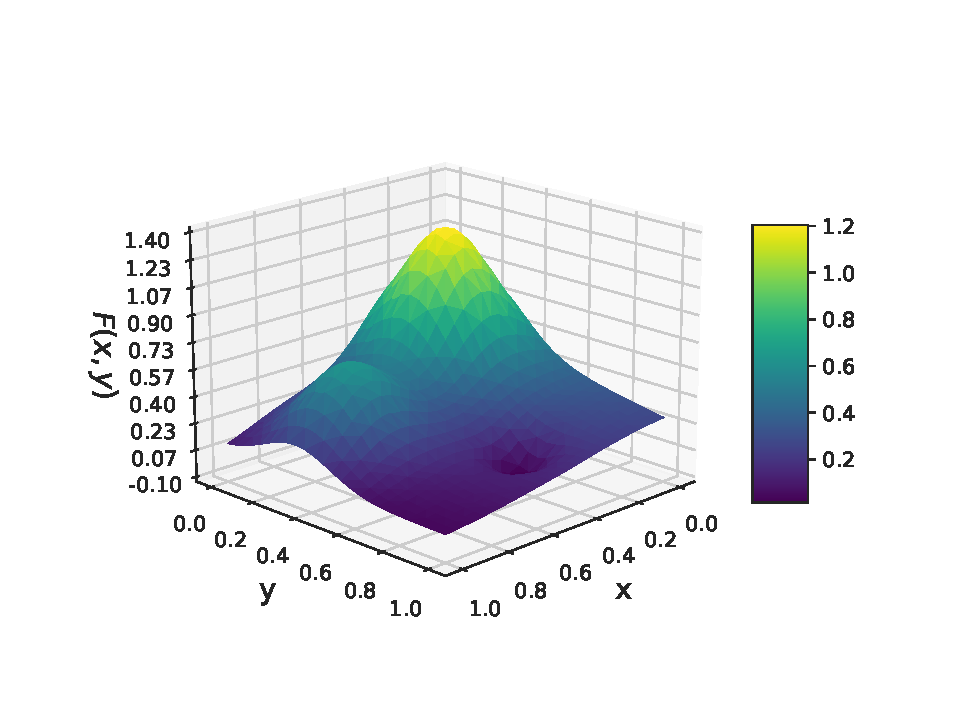
\includegraphics[width=\linewidth]{franke_functions_0.pdf}
        \caption{$\sigma = 0$}
        \end{subfigure}
        \hfill
        \begin{subfigure}{.5\textwidth}
        \centering
        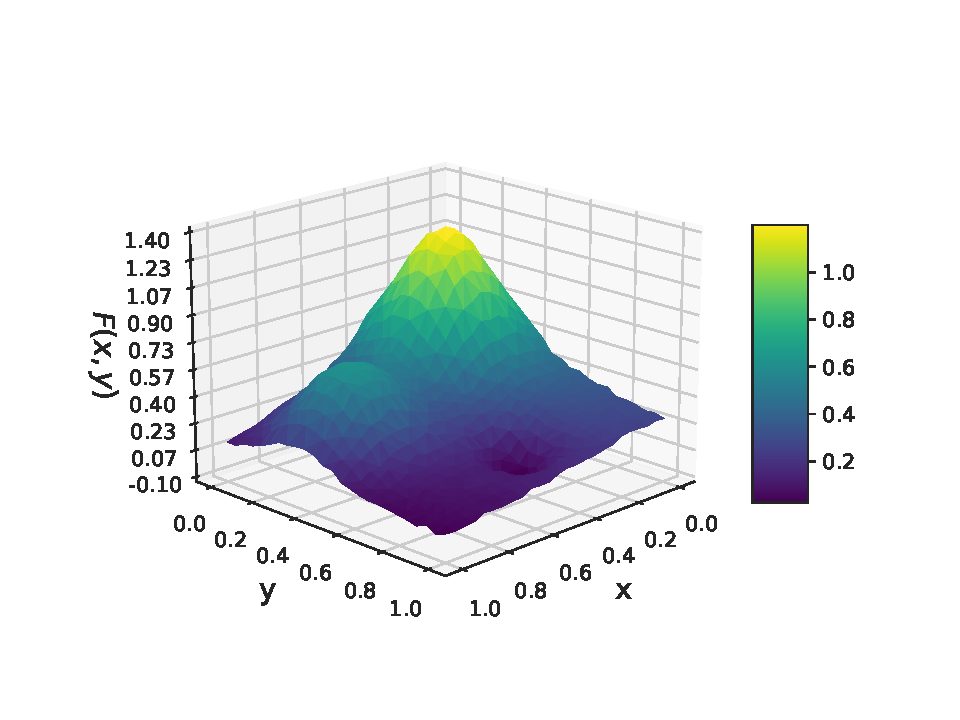
\includegraphics[width=\linewidth]{franke_functions_0_01.pdf}
        \caption{$\sigma = 0.01$}
        \end{subfigure}
        \hfill
        \begin{subfigure}{.5\textwidth}
        \centering
        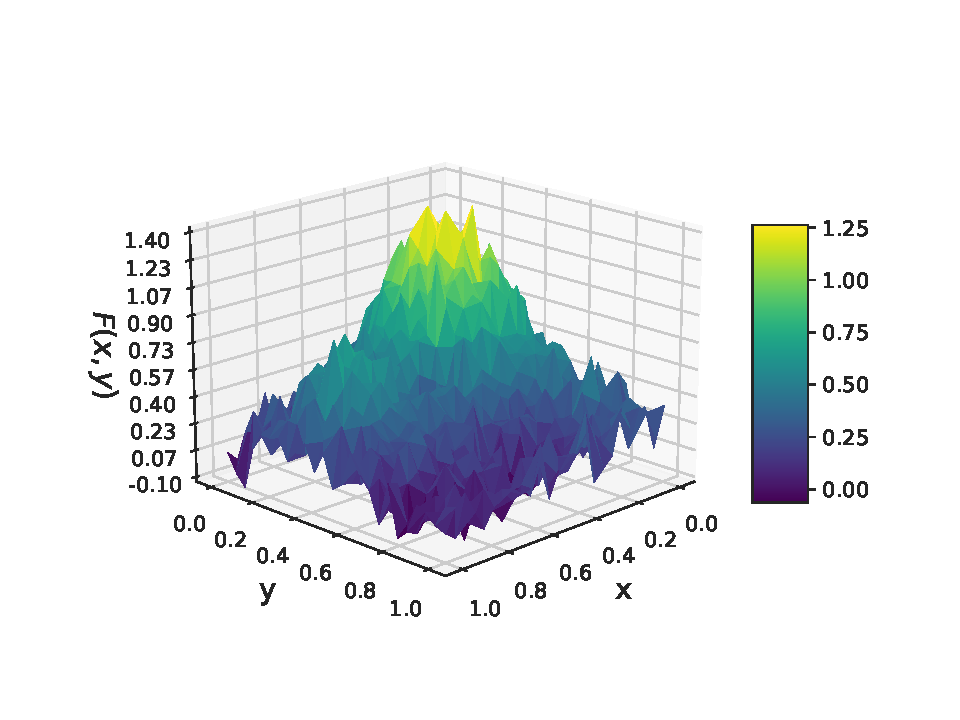
\includegraphics[width=\linewidth]{franke_functions_0_1.pdf}
        \caption{$\sigma = 0.1$}
        \end{subfigure}
        \begin{subfigure}{.5\textwidth}
        \centering
        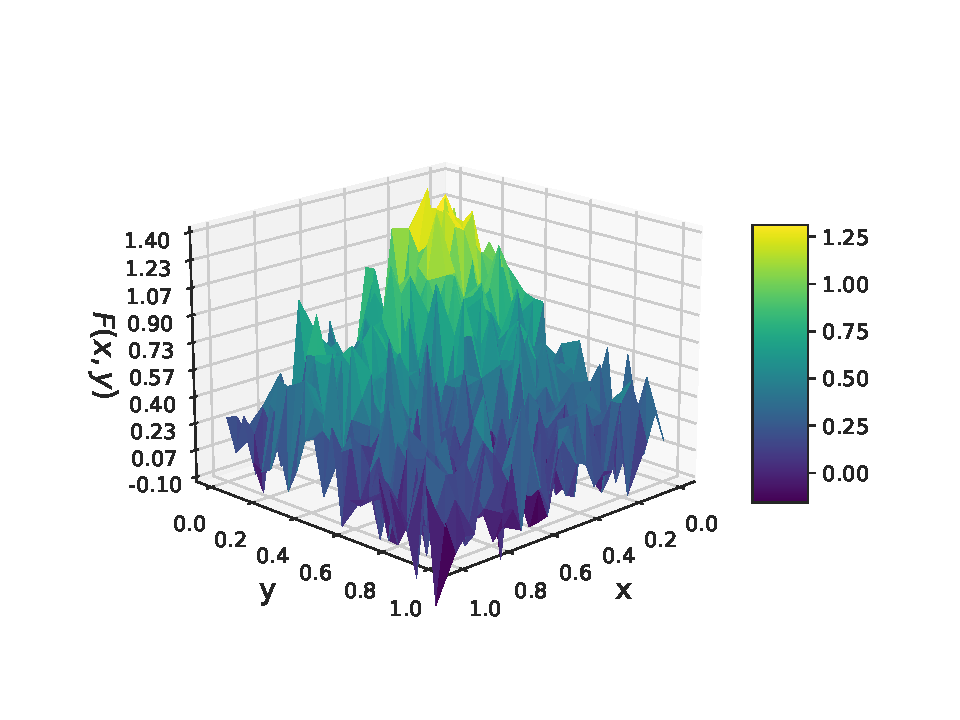
\includegraphics[width=\linewidth]{franke_functions_0_2.pdf}
        \caption{$\sigma = 0.2$}
        \end{subfigure}


        \centerline{Showing Franke function with increasing noise, from \textit{a} to \textit{d}, $\sigma \in \{ 0, 0.01, 0.1, 0.2\}$. All figures plotted with 625 equidistant $(x,y)$ points.}
    \end{figure*}


\end{appendix}

\printbibliography

\end{document}

